\documentclass[10pt,twocolumn,letterpaper]{article}

\usepackage{cvpr}
\usepackage{times}
\usepackage{epsfig}
\usepackage{graphicx}
\usepackage{amsmath}
\usepackage{amssymb}
\usepackage[inline]{enumitem}
\usepackage[numbers,sort]{natbib}
\usepackage{subcaption}
\usepackage{caption}

% Include other packages here, before hyperref.

% If you comment hyperref and then uncomment it, you should delete
% egpaper.aux before re-running latex.  (Or just hit 'q' on the first latex
% run, let it finish, and you should be clear).
\usepackage[breaklinks=true,bookmarks=false]{hyperref}

\cvprfinalcopy % *** Uncomment this line for the final submission

\def\cvprPaperID{****} % *** Enter the CVPR Paper ID here
\def\httilde{\mbox{\tt\raisebox{-.5ex}{\symbol{126}}}}
\providecommand{\keywords}[1]{\textbf{\textit{Index terms ---}} #1}

%\ifcvprfinal\pagestyle{empty}\fi
\setcounter{page}{1}
\begin{document}

\title{Image Inpainting Software}

\author{Yesheng Ma, Hu Hu, Yikai Zou\\
Shanghai Jiao Tong University\\
{\tt\small \{kimi.ysma, mihawkhu\}@gmail.com, zouyikai1014@163.com}
}

\maketitle
%\thispagestyle{empty}

\begin{abstract}
    Image inpainting is the technique to modifiy an image where the 
    inpainted area is unpredictable. There are already numerous methods
    introduced by former researchers to handle image inpainting including
    partial differential equations and Markov random fields. These methods
    all root in smoothing and have a immediate drawback of blurring.

    In this paper, we look deep into another kind of inpainting technique:
    examplar-based inpainting algorithm and further propose a method 
    inspired by the idea of priority queue. When we inpaint an image, we
    give different priority to the patches around the area to be inpainted
    and in this way we inpaint patches that capture the structure of the
    image better.

    Our experiments show that the idea of priority queue works well and
    is suitable for inpainting images with complex structure.
\end{abstract}

\keywords{Image Inpainting, Priority, Exemplar-Based Method}



\section{Introduction}

\subsection{Purpose of the project}
This project is the course project of software engineering at Shanghai
Jiao Tong University. The purpose of this project is to build a working
software for image inpainting. In this project specification, we will mainly
give the requirements specification, which includes 
\begin{enumerate*}
\item functional requirements
\item non-functional requirements
\item domain requirements
\end{enumerate*}; the software design, which includes 
\begin{enumerate*}
\item software model
\item software development tools
\item architectural design
\item object identification
\end{enumerate*}; testing, which includes
\begin{enumerate*}
\item test plan
\item test-design specification
\item test-case specification
\item test-procedure specification
\end{enumerate*}; as well as conclusion and references.


\subsection{Scope of the project}
\subsubsection{Project goal and task}
The goal and purpose of this project is shown as follows:
\begin{enumerate}
	\item Implement image in-painting algorithm. 
        When it is given an image and a chosen area, 
        it can remove the object in the area and inpaint the image.
    \item Both implement the project in a traditional manner and
        with a probabilistic graphical model, these two models should
        exhibit their benefits in different situations.
    \item Finally translate the prototype program into a GUI application
        with feasible user interaface, so that users can easily inpaint
        a target image.
\end{enumerate}
\subsubsection{Project cost}
In this project, there is no too much money cost needed for the 
exemplar-based method. However, in order to train that probabilitic
graphical model, i.e.\ Markov random field model, we need some number
of dataset. As we searched on the internet, there are not large dataset
for image inpainting and the only existing one is a dataset provided by
UC Berkeley with 300 inpainted images and we will use this dataset to
train the model.
\subsubsection{Schedule for this project}
The concreate timeline for this project is shown in the Table 1,
the deadline of this project is Jan 7, 2017.
\begin{table}
\hspace{-1cm}
\begin{tabular}{|c|c|c|}
\hline
Major Mission & Date & Finished or Not \\
\hline
Paper research, UML design, Requirement analysis
& 9/15 - 11/16& finished \\
\hline
Prototype design, paper proposal & 11/17 - 11/30 & finished \\
\hline
Backend development of exemplar-based algorithm & 12/1 - 12/11 & finished\\
\hline
Backend development of Markov random field & 12/11 - 12/25 & finished\\
\hline
Frontend development and user interface & 12/25 - 12/28 & finished\\
\hline
Test and refactoring & 12/28 - 1/3 &finished\\
\hline 
    final presentation & 1/4 - 1/4 & finished \\ \hline
    final report and paper writing & 1/4 - 1/6 & finished \\ \hline
\end{tabular}
\caption{Time schedule of this project}
\end{table}
\subsubsection{Hardware and software resources}
In this project, we have to deal with hardware and software resources since 
in a software development, these resources are critical.

Hardware:
\begin{enumerate}
\item Lab cluster to train MRF model
\item 3 laptops for software development
\end{enumerate}

Software:
\begin{enumerate}
\item use Python/MATLAB as backend programming language
\item use Python Tkinter cross platform GUI framework and MATLAB builtin
    GUI utility to build user interface
\end{enumerate}

\subsection{Overview}
In this final report, we will first talk about the requirement of image
inpainting. Image inpainting itself is as old as human art and it is really
a topic worth hard working. Actally, the image inpainting is quite useful
for ancient art museums.

Next, we will discuss the architecuture of this project in a software
enginnering manner. We will discuss why we design the image inpainting
system in that way and how we overcome the difficulties during developing
this system. We will also present some UML diagrams to illustrate our
design formally.

Also, we will talk about how our users can use this image inpainting 
software and what is the common work flow to use our image inpaiting
software. Although our user interface is quite user-friendly, users may
still be confused by the software since the technique we used to implement
image inpainting is quite complex.

Moreover, test specification is also given. Any modern reliable software
should be tested over multiple test cases and only in this way can our
software present  good reliability.

At last, we will conclude this project and give several topics for future
work since we find there might be more things we can discover in this
research field and we will give some references of this project.

\subsection{Development environment \& teamwork integration}
\subsubsection{Development environment}
We implemented two different algorithms: exemplar-based algorithm and
Markov random field in two platforms. We implemented the exemplar-based
algorithm on Windows 10 operating system and the MRF-based algorithm is
implemented on Ubuntu 16.04 Linux OS.

The proramming languages we use are carefully chosed. We use Python for
the exemplar-based algorithm since Python code is easy to write and there
are useful libraries like Tkinter, PIL, numpy, and scipy. We implement
the Markov random field algorithm in MATLAB since it is a machine learning,
to be specific a probabilistic graphical model, problem and we can use
MATLAB to easily implement matrix operations and some optimization
algorithms like SGD(stochastic gradient descent).
\subsection{Teamwork integration}
Since this is a quite large programming task and we work in a team to
contribute to this project, we decide to use Git version control system
to help us develop our project and actually we find we can further
save our source code on cloud for convenience and safety.

The most convenient component of GitHub might be the issue tracker. Once
a contributor discovers an issue, he can write a issue and another 
contributor can work on this issue and fix that bug. A sample issue is 
shown as follows:
\begin{figure}
    \centering
    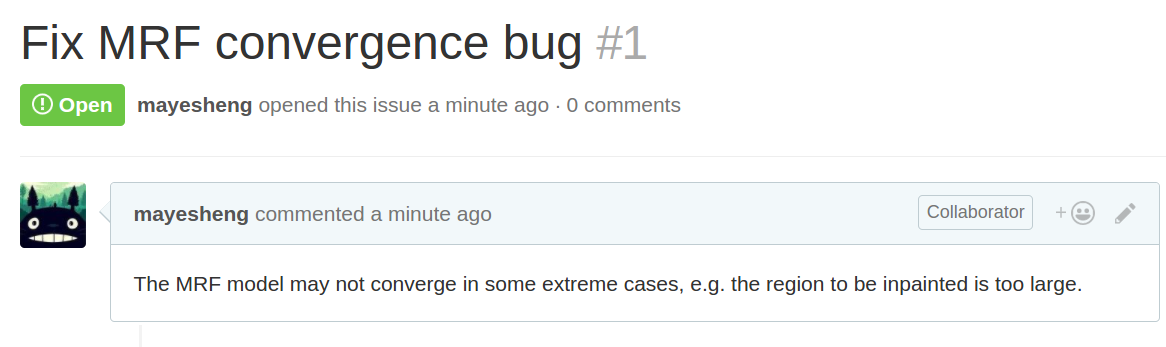
\includegraphics[width=10cm]{sc1.png}
    \caption{A sample issue tracker}
\end{figure}
Altogether we make about 50 commits and roughly 15000 lines of code.

\section{Related work and our contribution}
First we should make it clear that image inpainting and image denoising are
actually different tasks. In image inpainting, we aim to remove part of 
an image and a person needs to explicitly specify the area to be inpainted.
In constrast, as regard to image denoising, the task is to remove the 
``random'' noise of an image, which often does not need human supervison.
\subsection{Related work}
There are mainly two kinds of works on image inpainting: smoothing-based and
exemplar-based.

The research on image inpainting emerges on 2000, Marcelo Bertalmio \etal
\cite{siggraph00} first deals with the problem of image inpainting. Their
method is mainly based on intuition: propagate color information in the
direction of normal. However the limitation of the algorithm is that the
texture of its environment is unlikely to be reproduced.

Roth and Black \cite{cvpr05} later come up with a more general framework 
called \emph{Field of Experts} which is a Markov random field model. This
work relies on the result of Hinton \cite{neco02, nips02}, where Hinton discovers
that a factor in MRF can be modeled by a field of ``expert'' distributions.
In this work, they first learn the model and then apply the learned model
to Bertalmio's propagation method. Although this work in some sense captures
image structure, the blurring problem is also serious after our experiment. Later Bugeau\etal \cite{tip10} refined their result and optimize the execution time of the original method, but the problem of blurring is still there.

Another different way to tackle this problem is proposed by Criminisi \etal
 \cite{cvpr03,tip04}. They note that exemplar-based texture synthesis
 contains the essential process requred to replicate the structure of image.
 They introduce a priority for each exemplar and propagate according to
 the priority of each exemplar. This technique does not have the problem
 of blurring and can restore texture well, but may still fail for large
 object removal. Zongben Xu and Jian Sun also proposed a fix to the Criminisi's method in \cite{tip10sj}.

\subsection{Our contribution}
In this paper, we proposed a new way to define the priority of a patch 
around the boundary of a target region. We carefully design the priority of a patch to be the produce of two terms: the confidence term, data term and evaluation term.
The confidence term represents the amount of reliable information surrounding the pixel $p$. The data term represents the real line or margin information in image. Evaluation term represents the weight of each pixel in the target patch, which records the area of mask region in the target patch.

As is shown in the result analysis part, our algorithm can handle different size of mask and different kinds of textures. Also, our algorithm can be applied to image text removal, image object removal and image detail restoration, to name a few.

\section{Proposed methodology}
According to the discussion above, although there are existed work about the exemplar-based image inpainting algorithm \cite{cvpr03,tip04}. But previous attach a little too much calculation work to do when inpainting, it will result in long time to wait. Based on the previous work about exemplar-based image inpainting algorithm, we proposed a new evaluation criteria about the priority of each patch, which costs much less time than previous work and get good inpainted result.
\subsection{Two key observations}
\noindent \emph{A. Basic process unit size is important}

When select the exemplar region to inpaint the target region, the basic process unit size is important. The size of basic will effect the final result. Previous work has applied pixel as the basic unit\cite{iccv99}, the result will result in smoothing and blurring. It's easy to understand because small unit size ignore the connection between the each part of the image. Hence, we should not choose too small size of basic process unit. 

However, when the size of basic unit is too large, the target region inpainting will lead in to much difference. The large region of the mask region will get too much influence by the known region. That is to say, the target region will result in strange margin and line. So we should not choose too large basic process unit.

In our experiment, we test different unit size and compare them. Due to the difference of the number of calculation, process speed of each unit size is much different. Consider several factors, this algorithm present good results when the basic process size is $3*3$ or $5*5$.  Smaller size will result in smoothing and blurring, and larger size will result in unexpected disruption of target region. And in this paper, we will use patch as the name of the basic process unit.\\

\noindent \emph{B. Inpainting order is important}

When the image is inpainted by exemplar-based algorithm, the final result depends on the inpainting order selected by the algorithm. Some previous works randomly select the patch to inpaint, the result is worse than some previous works which select specific patch to do inpainting \cite{sivip16}. This section will demonstrate that the quality of
the output image synthesis is highly influenced by the order of the image inpainting. 
\begin{figure}
	\centering
	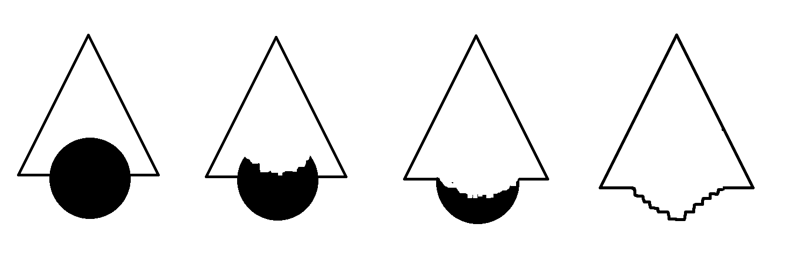
\includegraphics[width=0.94\linewidth]{order1.jpg}
	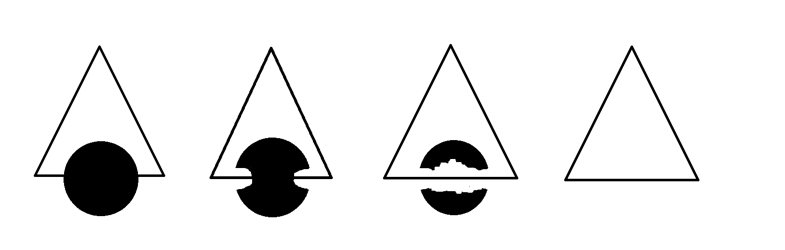
\includegraphics[width=1.0\linewidth]{order2.jpg}
	\caption{\textbf{The importance of the inpainting order}. The first group of images is the process of being inpainted from the up to the bottom, the second group of images is the process of being inpainted from the specific order.}
\end{figure}

In order to understand the importance of the inpainting order, a comparison between the specific order and fixed order is shown in Figure.1. the first group of images is using the up-to-bottom patch selection. Due to the target patch is always influenced by the nearby patch, so the bottom horizontal line of the triangle has not been inpainted. But if we do inpainting from the intersection of the target region and the bottom horizontal line, just as is shown in the second group of images. The horizontal line will be inpainted much better.

Therefore, a better image inpainting algorithm would be one that gives higher priority of synthesis to those regions of the target region which lie on
the continuation of image structures, as shown in the second group of Figure.1. 

\subsection{Our proposed method}
According to the two key observations mentioned above, the selection of patch that do inpainting first effects the final result much. So we should carefully select the specific patch. 
\begin{figure}
	\centering
	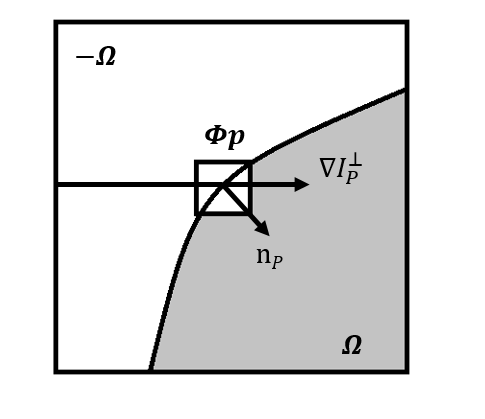
\includegraphics[width=0.94\linewidth]{region.jpg}
	\caption{\textbf{Notation figure}. The mask region and and the know region. The gradient and the unit vector is shown in the figure}
\end{figure}

Based on the image itself, in order to restore the original image, we should start from the intersection of the real line in image and the margin of the mask. So we use the dot cross result of the gradient and the unit vector orthogonal to the margin of the target region. Given a patch $\Phi_p$ centred at the point p for some $p \in \Omega$ (see Figure.2.), we define its priority $P(p)$ as the product of two terms:
\begin{equation*}
\centering
P(p)=C(p)*D(P)*A(p)
\nonumber
\end{equation*}

Where $C(p)$ is the confidence term of the patch $p$, $D(p)$ is the data term of the patch p, $E(p)$ is the evaluation term, which records the mask region in the target patch. 

Confidence term represents the amount of reliable information surrounding the pixel $p$. The
intention is to fill first those patches which have more of their pixels already inpainted, with additional preference given to pixels that were inpainted early on (or that were never part of the target region), it is calculated as follow:
\begin{equation*}
\centering
C(p)=\frac{\sum_{q\in \Phi _p\cap(-\Omega)}*C(q)}{|\Phi_p|}
\nonumber
\end{equation*}

Where $\Phi_p$ is the patch region, $|\Phi_p|$ is the area of the patch region. $\Omega$ is the target region, which is under the mask. $-\Omega$ is the region except for target region, it's the known region. During initialization, the confidence value is set to 1 in known region and 0 in mask region. 

Data term represents the real line or margin information in image. This factor is of
fundamental importance in our algorithm because it encourages linear structures to be synthesized first. It is the dot cross of the gradient and the unit vector orthogonal to the margin of the target region. It is calculated as follow:
\begin{equation*}
\centering
D(p)=\frac{|\nabla I^\bot_p \cdot n_p|}{\alpha}
\nonumber
\end{equation*}

Where $\nabla I^\bot_p$ is the gradient of image in pix $p$. $n_p$ is the unit vector orthogonal to the margin of the target region.

Evaluation term represents the weight of each pixel in the target patch, which records the area of mask region in the target patch. It is calculated as follow:
\begin{equation*}
\centering
E(p)=\frac{1}{\sum_{q \in \Phi_p \cap \Omega}q}
\nonumber
\end{equation*}

Where $\Phi_p$ is the patch region, $\Omega$ is the target region.

After defined the priority function of each patch, out algorithm work as the following steps.

First, given the input image and the input mask, initialize the whole patch in the margin with confidence term, data term and evaluation term. 

Next, compute the whole priority of each patch in mask margin, choose the maximum priority patch.

Then, traverse the patch that is near the target patch, compute the Euclidean distance of each pair of patch, find the exemplar patch minimizing the Euclidean distance.

Finally, copy the exemplar patch to the target patch where the pixel is unknown. And repeat these steps until there is no mask in the input image.

\subsection{Implementation details}
We implemented our algorithm in python. When we calculate the confidence term, data term and evaluation term, we used updated priority queue to operate data. It will save lots of time doing useless check and computing. 

We apply different size of patch and compare the result with each other. According to out experiment, patch size $3*3$ or $5*5$ will result in better result.

We assign normalization parameter $\alpha$ to 255 when we do inpainting. Due to the RGB form of our experiment images. It works well when assign any other significant value.

In all experiment, the size of mask was set to be larger than the patch size. And the image size is equal or larger than twice the mask size. Mask can be any shape.

We use a lot of images to test our algorithm, it may need much time when the mask is large, but it can successful handle different size of mask. Which is better than previous field of expert model \cite{ijcv09}, which will result in smoothing and blurring when mask size is large.

\section{Result and analysis}
Here we apply our algorithm to a variety of images, ranging from purely synthetic images to full-color photographs that include complex textures. According tor test result, our algorithm can handle different size of mask and different kinds of texture.

We test our algorithm in three scenarios, which includes image text removal, image object removal and image detail restoration. The following part will use some case to illustrate and analysis the result.

\subsection*{Image text removal}
In our daily life, we may often meet with image covered by text such as brand and advertisement. Given the mask which cover the whole text on the image, our algorithm can remove the text.

The example is shown in $Figure.3$, with the mask which cover the whole red text on the image, this algorithm will remove the whole red text. 
\begin{figure}
	\centering
	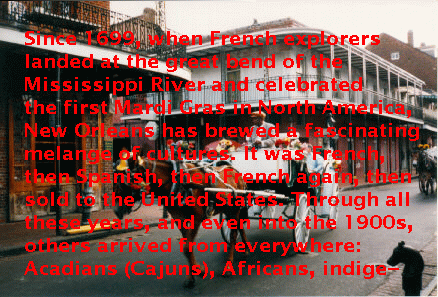
\includegraphics[width=0.9\linewidth]{horse_car.png}\\\ \\
	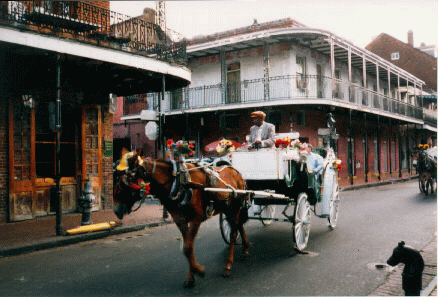
\includegraphics[width=0.9\linewidth]{horse_car_result.png}
	\caption{\textbf{Image text removal}. The original image and inpainted image}
\end{figure}

\subsection*{Image object removal}
Compared with previous field model \etal\cite{cvpr10mrf, ijcv09}, which can not handle large mask well, our algorithm can successfully inpainting large mask. The result is shown in the $Figure.4$. 
\begin{figure}
	\centering
	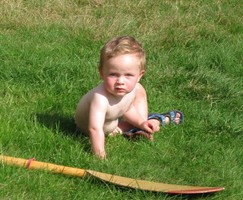
\includegraphics[width=0.9\linewidth]{kid.jpg}\\\ \\
	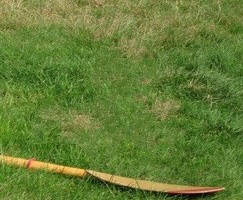
\includegraphics[width=0.9\linewidth]{kid_result.jpg}
	\caption{\textbf{Image object removal}. The original image and inpainted image}
\end{figure}

\subsection*{Image detail restoration}
We may get some disrupted images such as old photos. The result of the image detail restoration is shown in $Figure.5$. If observed inpainted image carefully, you may find some inpainting trace on it, but it dose not matter for the final result. As the result shows, it works well.
\begin{figure}
	\centering
	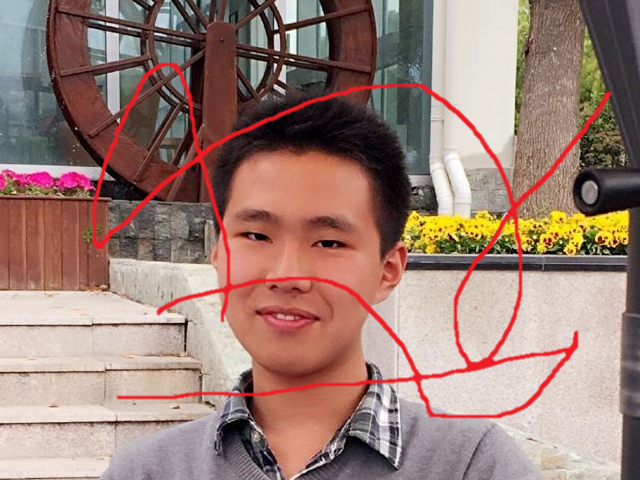
\includegraphics[width=0.9\linewidth]{zouyikai.png}\\\ \\
	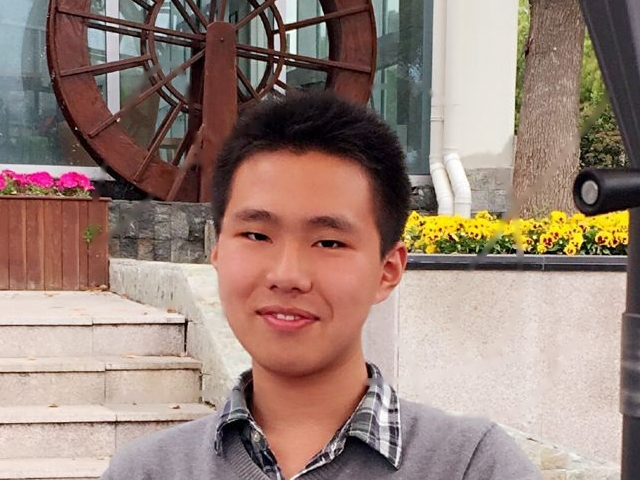
\includegraphics[width=0.9\linewidth]{zouyikai_result.png}
	\caption{\textbf{Image detail restoration}. The original image and inpainted image}
\end{figure}
\section{Conclusion and future work}
This paper has presented a novel algorithm for image inpainting. The result is an image in
which the selected object has been replaced by a visually plausible background that mimics the appearance of the source region. Given the mask region and input image, our algorithm can do image inpainting and get good result as shown in this paper. 

Our algorithm is capable of different size of input mask and can apply to different kinds of scenarios including image text removal, image object removal and image detail restoration. Our method can successfully solve these problem efficiently.

In the future, we plan to increase the process speed and get better image inainting result. Also, we plan to try some new model such as deep learning model on topic. We plan to set up an estimate of the result, which can get more directly comparing result of different image inpainting method.

\section{Acknowledgements}
We got a lot of help from my Software Engineering teacher Professor Sheng Bin while we are writing the paper. He had given us appropriate example and knowledge in order to make us understand more about this Software Engineering study. We faced many problems during coding and writing but our teaching assistant always companies with us. So we also appreciate the teaching assistants Saleha Masood. Saleha has a meeting with us every two weeks. She spends her time to find information for us to carry out the project. Also thanks other groups which willing to share their information about Software Engineering study. They give us a lot if new ideas about the project.

\newpage
{\small
\bibliographystyle{ieee}
\bibliography{paper}
}

\end{document}
